\label{chap:system-arch}
With the requirement specification, defined in section \ref{sec:moscow}, the design of the system has now been defined and described. The first step for this is to define the over all system architecture. 

The architecture were formally defined using UML diagrams. The first step in designing the architecture were to explore the different components that make up the system. After this, the system criteria were evaluated for each component. 

From these the design is then formalized for each component and described.

\section{Components}
Based on the arguments of chapter \ref{chap:technologies}, the system has been split into different components, with different responsibilities. Since the system should implement different technologies all running on different platforms, it was decided to connect it all through a web service. This would make it possible to connect new components to the solution which could expand on the functionality of the solution. In this section the different components has been described and in the end defined with use of class diagrams.

\begin{figure}[H]
    \centering
    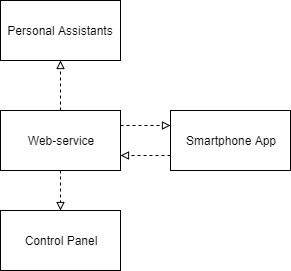
\includegraphics[width=0.4\textwidth]{Figures/deploymentdiagram.png}
    \caption{Component Diagram}
    \label{fig:componentsDiagram}
\end{figure}

On figure \ref{fig:componentsDiagram} the connections between the different components of the system are shown. All components will communicate with the web service through models, and the web service will communicate with the app through the use of notifications.

\subsection{Smartphone app}
The functionality of the smartphone app has been separated into two components, one for citizens, and one for contacts. The first component is used to activate an alarm, when a fall accident has occurred. As mentioned in section \ref{sec:moscow} automatic fall detection has not been considered. As a result of this, a citizen must activate the alarm manually. When activating an alarm, the citizen should still have a chance to cancel the alarm in case it was a false positive. 

The second component of the smartphone app is used by a contact. When a citizen has raised an alarm, and the system tries to contact the contact person, they receive a notification. The contact person can then answer the alarm, to let the system know if they are able to help or not. 

All interaction for the app for both components happens through the web service where login, creating and updating an alarm takes place. The app should not have any functionality when the user is not logged in.

\subsection{Personal assistant}\label{sec:personalAssistant}
The personal assistant will allow the citizen to call for help by uttering a few words. These words should be clear and logical for the user, but not allow for false positives, that could occur during normal conversation. When the personal assistant has confirmed that the citizen has had a falling accident, it notifies the web service, and creates the alarm. 

\subsection{Web service}
The web service is the central part of the system, where all computations are done and all communication between the different components happen. The web service is accessible through a web API. When the web service receives an alarm from a citizens device, it is responsible for making contact to the different contacts associated with the citizen that has had the fall accident, and report back to the citizen when a contact has responded to the alarm.

\subsection{Control panel}
The control panel is used to manage users and their associated information. From it, it is possible to create new citizens, define their contact-list, devices, and manage their login information. It should be separated from the rest of the system, as to avoid confusion that could lead to unwanted changes.

\section{System criteria}
\label{sec:non-requirements}
The system criteria has been defined for each component. These functions are used as guidelines during the design of the system architecture. The different criteria that is used are from the book \textit{Objekt orienteret analyse \& design} \cite{subook}.


\begin{table}[H]
\centering
\begin{tabular}{|l|c|c|c|c|}
\hline
              & \multicolumn{1}{l|}{Smartphone app} & \multicolumn{1}{l|}{Personal assistant} & \multicolumn{1}{l|}{Web service} & \multicolumn{1}{l|}{Control panel} \\ \hline
Usable        & x                                   & x                                &                              & x                                  \\ \hline
Secure        &                                     &                                  & x                            & x                                  \\ \hline
Efficient     & x                                   &                                  & x                            &                                    \\ \hline
Correct       & x                                   & x                                & x                            & x                                  \\ \hline
Reliable      & x                                   & x                                & x                            &                                    \\ \hline
Maintainable  &                                     &                                  & x                            &                                    \\ \hline
Testable      & x                                   & x                                & x                            &                                    \\ \hline
Flexible      &                                     &                                  & x                            &                                    \\ \hline
Comprehensive &                                     &                                  &                              &                                    \\ \hline
Reuseable     &                                     &                                  &                              &                                    \\ \hline
Portable      & x                                   &                                  &                              &                                    \\ \hline
Interoperable &                                     &                                  & x                            &                                    \\ \hline
\end{tabular}
\caption{System criteria}
\label{tab:non-functional}
\end{table}

The most important criteria for each component are as seen on figure \ref{tab:non-functional}. Each decision has been elaborated further in this section.

\paragraph{Usable}
Usability is an important aspect for this solution, since it will be used by citizens that often do not have much experience with technology. This is reflected in the different components of the system. The only component that does not need to have a high degree of usability is the web service, since this does not have a direct way to interact with it.

The control panel should be simple, such that the citizen admins easily can manage the citizens, contacts and devices.

The smartphone app should be simple to make it easy to use for citizens, in case they have a fall accident.

The personal assistant will be communicating with the citizen. The interaction between personal assistant and citizen should be simple, such that the citizen can manage the conversation, even in a state of panic that might occur during or after a fall accident.

\paragraph{Secure}
It is important for the web service and control panel to be secure as they allow access to personal information for the different users.

Since the smartphone app and the personal assistant would not have access to such data, there is no need to implement further security measures, than what their respective platforms offer. Communication regarding passwords and usernames should still be encrypted.

\paragraph{Efficient}
The efficiency of the smartphone app is important due to concerns about power usage. The app would be constantly running, and could therefore be draining the battery if not implemented in an efficient manner. The efficiency of the web service is important, such that it can handle any amount of simultaneous requests.

\paragraph{Correct}
Every part of the system needs to fulfill the specified requirements.

\paragraph{Reliable}
The smartphone app must be able to perform fall detection with such precision, that it does not create any false negatives.

The personal assistant must be able to perform its voice recognition with such precision, that it does not create false negatives.

The web service needs to be reliable, such that it does not corrupt data. This could for example be that it does not give out the wrong data when a request is made for user data, or send out wrong notifications regarding falling accidents. It also should never lose data.

\paragraph{Maintainable}
The web service needs to be maintainable, such that it is possible to integrate devices, such as different IoT device, in the future, without a need to rewrite the web service every time a device is added or removed.

\paragraph{Testable}
It is important that the smartphone app, personal assistant and web service are thoroughly tested. If a component malfunctions when it is needed, the citizen will not receive the needed help. Therefore they all need to be highly testable.

\paragraph{Flexible}
The web service must be flexible, such that it is possible, and economically feasible, to change parts of the Web-Service after it has been taken into use.

\paragraph{Comprehensive}
Because of the simplicity of the different parts of the system, this is trivially achieved for all components, and is therefore not an important criteria.

\paragraph{Reusable}
There will be no focus on making any of the components in the system reusable.

\paragraph{Portable}
The smartphone app must be written in a way that makes it easy to port to a new platform, such that it is possible to use on any smartphone a user might have.

\paragraph{Interoperable}
The web service must be able to integrate with new devices without it requiring expensive changes to the web service. This enables possible future extension of the system.
